\documentclass[journal,12pt,twocolumn]{IEEEtran}

\usepackage{setspace}
\usepackage{gensymb}

\singlespacing


\usepackage[cmex10]{amsmath}

\usepackage{amsthm}

\usepackage{mathrsfs}
\usepackage{txfonts}
\usepackage{stfloats}
\usepackage{bm}
\usepackage{cite}
\usepackage{cases}
\usepackage{subfig}

\usepackage{longtable}
\usepackage{multirow}

\usepackage{enumitem}
\usepackage{mathtools}
\usepackage{steinmetz}
\usepackage{tikz}
\usepackage{circuitikz}
\usepackage{verbatim}
\usepackage{tfrupee}
\usepackage[breaklinks=true]{hyperref}
\usepackage{graphicx}
\usepackage{tkz-euclide}

\usetikzlibrary{calc,math}
\usepackage{listings}
    \usepackage{color}                                            %%
    \usepackage{array}                                            %%
    \usepackage{longtable}                                        %%
    \usepackage{calc}                                             %%
    \usepackage{multirow}                                         %%
    \usepackage{hhline}                                           %%
    \usepackage{ifthen}                                           %%
    \usepackage{lscape}     
\usepackage{multicol}
\usepackage{chngcntr}

\DeclareMathOperator*{\Res}{Res}

\renewcommand\thesection{\arabic{section}}
\renewcommand\thesubsection{\thesection.\arabic{subsection}}
\renewcommand\thesubsubsection{\thesubsection.\arabic{subsubsection}}

\renewcommand\thesectiondis{\arabic{section}}
\renewcommand\thesubsectiondis{\thesectiondis.\arabic{subsection}}
\renewcommand\thesubsubsectiondis{\thesubsectiondis.\arabic{subsubsection}}


\hyphenation{op-tical net-works semi-conduc-tor}
\def\inputGnumericTable{}                                 %%

\lstset{
%language=C,
frame=single, 
breaklines=true,
columns=fullflexible
}
\begin{document}


\newtheorem{theorem}{Theorem}[section]
\newtheorem{problem}{Problem}
\newtheorem{proposition}{Proposition}[section]
\newtheorem{lemma}{Lemma}[section]
\newtheorem{corollary}[theorem]{Corollary}
\newtheorem{example}{Example}[section]
\newtheorem{definition}[problem]{Definition}

\newcommand{\BEQA}{\begin{eqnarray}}
\newcommand{\EEQA}{\end{eqnarray}}
\newcommand{\define}{\stackrel{\triangle}{=}}
\bibliographystyle{IEEEtran}

\providecommand{\mbf}{\mathbf}
\providecommand{\pr}[1]{\ensuremath{\Pr\left(#1\right)}}
\providecommand{\qfunc}[1]{\ensuremath{Q\left(#1\right)}}
\providecommand{\sbrak}[1]{\ensuremath{{}\left[#1\right]}}
\providecommand{\lsbrak}[1]{\ensuremath{{}\left[#1\right.}}
\providecommand{\rsbrak}[1]{\ensuremath{{}\left.#1\right]}}
\providecommand{\brak}[1]{\ensuremath{\left(#1\right)}}
\providecommand{\lbrak}[1]{\ensuremath{\left(#1\right.}}
\providecommand{\rbrak}[1]{\ensuremath{\left.#1\right)}}
\providecommand{\cbrak}[1]{\ensuremath{\left\{#1\right\}}}
\providecommand{\lcbrak}[1]{\ensuremath{\left\{#1\right.}}
\providecommand{\rcbrak}[1]{\ensuremath{\left.#1\right\}}}
\theoremstyle{remark}
\newtheorem{rem}{Remark}
\newcommand{\sgn}{\mathop{\mathrm{sgn}}}
\providecommand{\abs}[1]{\left\vert#1\right\vert}
\providecommand{\res}[1]{\Res\displaylimits_{#1}} 
\providecommand{\norm}[1]{\left\lVert#1\right\rVert}
%\providecommand{\norm}[1]{\lVert#1\rVert}
\providecommand{\mtx}[1]{\mathbf{#1}}
\providecommand{\mean}[1]{E\left[ #1 \right]}
\providecommand{\fourier}{\overset{\mathcal{F}}{ \rightleftharpoons}}
%\providecommand{\hilbert}{\overset{\mathcal{H}}{ \rightleftharpoons}}
\providecommand{\system}{\overset{\mathcal{H}}{ \longleftrightarrow}}
	%\newcommand{\solution}[2]{\textbf{Solution:}{#1}}
\newcommand{\solution}{\noindent \textbf{Solution: }}
\newcommand{\cosec}{\,\text{cosec}\,}
\providecommand{\dec}[2]{\ensuremath{\overset{#1}{\underset{#2}{\gtrless}}}}
\newcommand{\myvec}[1]{\ensuremath{\begin{pmatrix}#1\end{pmatrix}}}
\newcommand{\mydet}[1]{\ensuremath{\begin{vmatrix}#1\end{vmatrix}}}

\numberwithin{equation}{subsection}

\makeatletter
\@addtoreset{figure}{problem}
\makeatother
\let\StandardTheFigure\thefigure
\let\vec\mathbf

\renewcommand{\thefigure}{\theproblem}

\def\putbox#1#2#3{\makebox[0in][l]{\makebox[#1][l]{}\raisebox{\baselineskip}[0in][0in]{\raisebox{#2}[0in][0in]{#3}}}}
     \def\rightbox#1{\makebox[0in][r]{#1}}
     \def\centbox#1{\makebox[0in]{#1}}
     \def\topbox#1{\raisebox{-\baselineskip}[0in][0in]{#1}}
     \def\midbox#1{\raisebox{-0.5\baselineskip}[0in][0in]{#1}}
\vspace{3cm}
\title{Assignment 2}
\author{Sachinkumar Dubey}

\maketitle
\newpage

\bigskip
\renewcommand{\thefigure}{\theenumi}
\renewcommand{\thetable}{\theenumi}
Download all python codes from 
\begin{lstlisting}
https://github.com/sachinomdubey/Matrix-theory/Assignment2/codes
\end{lstlisting}
%
and latex-tikz codes from 
%
\begin{lstlisting}
https://github.com/sachinomdubey/Matrix-theory/Assignment2
\end{lstlisting}
%

\noindent Q no. 73. Find the angle between the following pair of lines: Also find the closest points and minimum distance between them.
\begin{enumerate}
\item
\begin{align}
L_1: \quad \vec{x} &= \myvec{2\\-5\\1} + \lambda_1\myvec{3 \\ 2 \\6}
\\
L_2: \quad \vec{x} &= \myvec{7\\-6\\0} + \lambda_2\myvec{1 \\ 2 \\2}
\end{align}
\item
\begin{align}
L_1: \quad \vec{x} &= \myvec{3\\1\\-2} + \lambda_1\myvec{1 \\ -1 \\-2}
\\
L_2: \quad \vec{x} &= \myvec{2\\-1\\-56} + \lambda_2\myvec{3 \\ -5 \\-4}
\end{align}
\end{enumerate}
%
\\
\solution 
\begin{enumerate}
\item The direction vectors of the lines are
\myvec{3 \\ 2 \\6} and \myvec{1 \\ 2 \\2}. \\
Thus, the angle $\theta$ between two vectors is given by 
%
\begin{align}
\label{eq:line_scalar_prod}
\cos \theta &= \frac{\vec{a}^T\vec{b}}{\norm{\vec{a}}\norm{\vec{b}}}
\\
&=\frac{19}{3\times7}
\\
\implies \theta &= 25.21\degree
\end{align}
\item The direction vectors of the lines are
\myvec{1 \\ -1 \\-2} and \myvec{3 \\ -5 \\-4}. \\
Thus, the angle $\theta$ between two vectors is given by 
%
\begin{align}
\label{eq:line_scalar_prod}
\cos \theta &= \frac{\vec{a}^T\vec{b}}{\norm{\vec{a}}\norm{\vec{b}}}
\\
&=\frac{16}{\sqrt6\times\sqrt50}
\\
\implies \theta &= 22.52\degree
\end{align}
\end{enumerate} 
\\
\textbf{Note :} In both problems, the respective pair of lines do not intersect each other (called skew lines), The obtained angle is the angle between the direction vectors of the lines. The proof that the pair of lines do not intersect in Problem 1 is as follows:\\
\\
\textbf{Problem 1 :} Equating the x, y and z components of both lines and forming equation in the augmented matrix form. The Matrix is row reduced as follows:
\begin{align}
\myvec{3 & -1 & 5\\2 & -2 & -1\\6 &-2&-1}\\
\xleftrightarrow[]{R_1\leftarrow R_1/3}
\myvec{3 & -1/3 & 5/3 \\2 & -2 & -1\\6 &-2&-1}\\
\xleftrightarrow[]{R_2\leftarrow R_2-2R_1}   
\myvec{3 & -1/3 & 5/3\\0 & -4/3 & -13/3\\6 &-2&-1}\\
\xleftrightarrow[]{R_3\leftarrow R_3-6R_1}
\myvec{3 & -1/3 & 5/3\\0 & -4/3 & -13/3\\0 &0&-11}
\end{align} 
Here, Rank(A) $\neq$ Rank(A$\mid$B). Hence, these three equations are inconsistent, which proves that the two lines do not intersect in the 3D plane. (Where A is the coefficient matrix and A$\mid$B is the augmented matrix.) \\
\\
\textbf{Finding the closest points on the lines and minimum distance (Problem 1) :}
\\
The given equations are in the form:
\begin{align}
    \textbf{x}=\vec{p_1} + \lambda_1\vec{d_1}\\
    \textbf{x}=\vec{p_2} + \lambda_2\vec{d_2}
\end{align}
Where, $\vec{p_1}$ and $\vec{p_2}$ are points on line1 and line2 respectively. Also, $\vec{d_1}$ and $\vec{d_2}$ are the direction vectors of respective lines.
The cross product of $\vec{d_1}$ and $\vec{d_2}$ is perpendicular to both lines.
\begin{align}
    \vec{n} = \vec{d_1} \times \vec{d_2}\\
     \vec{n}=\myvec{4-8 \\ -(6-6) \\ 6-2}
     \implies \vec{n}=\myvec{-8 \\ 0 \\ 4}
\end{align}
\\
When the line2 is translated along the vector \vec{n}, it forms a plane. This plane intersects line1 at a single point $\vec{c_1}$ which is nearest to the line2. Point $\vec{c_1}$ is given by:
\\
\begin{align}
\vec{c_1}=\vec{p_1}+\frac{(\vec{p_2}-\vec{p_1})^T \vec{n_2}}{\vec{d_1}^T \vec{n_2}}\vec{d_1} \\
where, \vec{n_2}=\vec{d_2}\times \vec{n}\\
 \therefore \vec{n}=\myvec{8-0 \\ -(4+16) \\ 0+16}
\implies \vec{n_2}=\myvec{8 \\ -20 \\ 16}\\
\therefore \vec{c_1}= \myvec{2\\-5\\1}+\frac{\myvec{5&-1&-1} \myvec{8\\-20\\16}}{\myvec{3&2&6} \myvec{8\\-20\\16}}\myvec{3\\2\\6}\\
\implies \vec{c_1}=\myvec{3.65\\-3.9\\4.3}
\end{align}
Similarly, the point on Line2 nearest to Line 1 is $\vec{c_2}$ given by:\\
\begin{align}
\vec{c_2}=\vec{p_2}+\frac{(\vec{p_1}-\vec{p_2})^T \vec{n_1}}{\vec{d_2}^T \vec{n_1}}\vec{d_2} \\
where, \vec{n_1}=\vec{d_1}\times n\\
 \therefore \vec{n}=\myvec{8-0 \\ -(12+48) \\ 0+16}
\implies \vec{n_1}=\myvec{8 \\ -60 \\ 16}
\end{align}
\begin{align}
\therefore \vec{c_2}= \myvec{7\\-6\\0}+\frac{\myvec{-5&1&1} \myvec{8\\-60\\16}}{\myvec{1&2&2} \myvec{8\\-60\\16}}\myvec{1\\2\\2}\\
\implies \vec{c_2}=\myvec{8.05\\-3.9\\2.1}
\end{align}
\\
The minimum distance can be found using points $\vec{c_1}$ and $\vec{c_2}$ as \textbf{4.92} units.
\begin{figure}[ht]
\centering
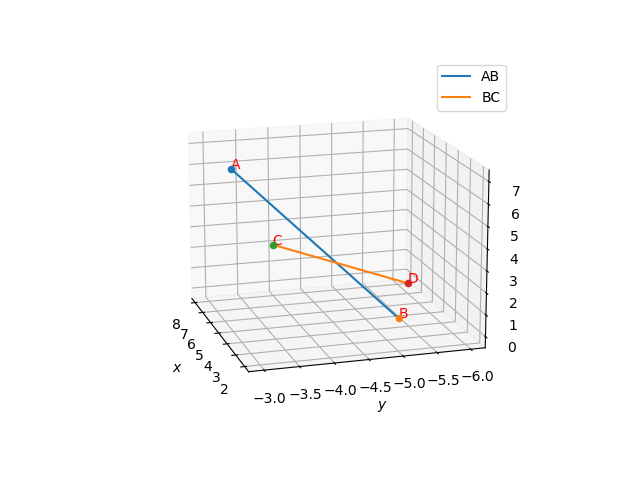
\includegraphics[width=10cm, height=8cm]{Figure_1}
\caption{Problem 1 : Lines crossing each other, but not intersecting}
\label{Fig2}
\end{figure}
\newpage
The proof that the pair of lines do not intersect in Problem 2 is as follows:\\
\\
\textbf{Problem 2 :} Equating the x, y and z components of both lines and forming equation in the augmented matrix forms. The Matrix is row reduced as follows:\\
\begin{align}
\myvec{1 & -3 & -1\\-1 & 5 & -2\\-2 &4&-54}\\
\xleftrightarrow[]{R_2\leftarrow R_2+R_1}
\myvec{1 & -3 & -1 \\0 & 2 & -3\\-2 &4&-54}\\
\xleftrightarrow[]{R_3\leftarrow R_3+2R_1}   
\myvec{1 & -3 & -1 \\0 & 2 & -3\\0 &-2&-56}\\
\xleftrightarrow[]{R_2\leftarrow R_2/2}
\myvec{1 & -3 & -1 \\0 & 1 & -3/2\\0 &-2&-56}\\
\xleftrightarrow[]{R_3\leftarrow R_3+2R_2}
\myvec{1 & -3 & -1 \\0 & 1 & -3/2\\0 &0&-59}
\end{align} 
Here, Rank(A) $\neq$ Rank(A$\mid$B).
\\
Hence, the equations are inconsistent, which proves that the two lines do not intersect in the 3D plane. (Where A is the coefficient matrix and A$\mid$B is the augmented matrix.) \\
\\
\noindent
\textbf{Finding the closest points on the lines and minimum distance (Problem 2) :}\\
\\
The given equations are in the form:
\begin{align}
    \textbf{x}=\vec{p_1} + \lambda_1\vec{d_1}\\
    \textbf{x}=\vec{p_2} + \lambda_2\vec{d_2}
\end{align}
Where, $\vec{p_1}$ and $\vec{p_2}$ are points on line1 and line2 respectively. Also, $\vec{d_1}$ and $\vec{d_2}$ are the direction vectors of respective lines.
The cross product of $\vec{d_1}$ and $\vec{d_2}$ is perpendicular to both lines.
\begin{align}
    \vec{n} = \vec{d_1} \times \vec{d_2}\\
    \vec{n}=\myvec{4-10 \\ -(-4+6) \\ -5+3}
     \implies \vec{n}=\myvec{-6 \\ -2 \\ -2 }
\end{align}
\\
When the line2 is translated along the vector \vec{n}, it forms a plane. This plane intersects line1 at a single point $\vec{c_1}$ which is nearest to the line2. Point $\vec{c_1}$ is given by:
\\
\begin{align}
\vec{c_1}=\vec{p_1}+\frac{(\vec{p_2}-\vec{p_1})^T \vec{n_2}}{\vec{d_1}^T \vec{n_2}}\vec{d_1} \\
where, \vec{n_2}=\vec{d_2}\times \vec{n}\\
 \therefore \vec{n_2}=\myvec{10-8 \\ -(-6-24) \\ -6-30}
\implies \vec{n_2}=\myvec{2 \\ 30 \\ -36}\\
\vec{c_1}= \myvec{3\\-1\\-2}+\frac{\myvec{-1&-2&-54} \myvec{2\\30\\-36}}{\myvec{1&-1&-2} \myvec{2\\30\\-36}}\myvec{1\\-1\\-2}\\
\implies \vec{c_1}=\myvec{45.77 \\ -41.77\\ -87.54}
\end{align}
Similarly, the point on Line2 nearest to Line 1 is $\vec{c_2}$ given by:\\
\begin{align}
\vec{c_2}=\vec{p_2}+\frac{(\vec{p_1}-\vec{p_2})^T \vec{n_1}}{\vec{d_2}^T \vec{n_1}}\vec{d_2} \\
where, \vec{n_1}=\vec{d_1}\times \vec{n}\\
 \therefore \vec{n_1}=\myvec{2-4 \\ -(-2-12) \\ -2-6}
\implies \vec{n_1}=\myvec{-2 \\ 14 \\ -8}
\end{align}
\begin{align}
\therefore \vec{c_2}= \myvec{2\\-1\\-56}+\frac{\myvec{5&-1&-1} \myvec{-2\\14\\-8}}{\myvec{3&-5&-4} \myvec{-2\\14\\-8}}\myvec{3\\-5\\-4}\\
\implies \vec{c_2}=\myvec{29.69\\ -47.15\\ -92.92}
\end{align}
\\
The minimum distance can be found using points $\vec{c_1}$ and $\vec{c_2}$ as \textbf{17.79} units.
\newpage
\begin{figure}[h!]
\centering
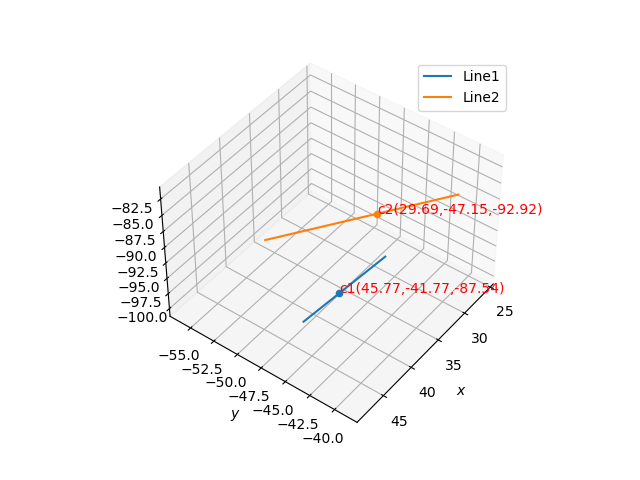
\includegraphics[width=10cm, height=8cm]{Figure_2}
\caption{Problem 2 : Lines crossing each other, but not intersecting}
\label{Fig4}
\end{figure}
\end{document}